\section{Adam Tokarz}

1) Wyrażenia matematyczne:

\begin{center}
    \begin{equation}
        f(x)=\sqrt{x+4}+\log_{2}({x^{3}+8})
    \end{equation}
    \begin{equation}
        V_{n}^{k}=\frac{n!}{(n-k)!}
    \end{equation}
\end{center}

2) Zdjęcie zachodu Słońca: (Figure~\ref{fig:sunset})
\begin{figure} [htbp]
    \centering
    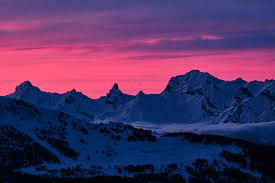
\includegraphics[scale=0.75]{pictures/sunset.jpg}
    \caption{Zachód Słońca w górach}
    \label{fig:sunset}
\end{figure}


3) Tabela:~\ref{tab:my_tabela}
\begin{table}[htbp]
    \centering
   \begin{tabular}{|c|c|c|c|}
\hline
           & \textbf{A} & \textbf{B} & \textbf{C} \\ \hline
\textbf{1} & A1         & B1         & C1         \\ \hline
\textbf{2} & A2         & B2         & C2         \\ \hline
\textbf{3} & A3         & B3         & C3         \\ \hline
\textbf{4} & A4         & B4         & C4         \\ \hline
    \end{tabular}
    \caption{Tabela 4x3}
    \label{tab:my_tabela}
\end{table}
    





4) Lista numerowana:
\begin{enumerate}
    \item item1
    \item item2
    \item item3
\end{enumerate}

5) Lista nienumerowana:
\begin{itemize}
    \item item
    \item other item
    \item another item
\end{itemize}

\begin{itemize}
    \item[-] pauza
    \item[!] wykrzyknik
    \item[$\blacksquare$] czarny kwadrat
\end{itemize}

6) Krótki tekst z podstawowym formatowaniem:

\textbf{Wenus, jako jedyna planeta w Układzie Słonecznym, obraca się wstecznie do kierunku Słońca.} Ponadto jej obrót wokół własnej osi, zachodzący w ciągu 243 dni, trwa dłużej niż obrót wokół Słońca (225 dni). \underline{Oznacza to, że na tej planecie jeden dzień jest dłuższy niż jeden rok.}

Chociaż na Ziemi obserwujemy wyłącznie opady wody (pod rozmaitymi postaciami), w przypadku innych planet sprawa przedstawia się zgoła inaczej. \textit{Na Wenus z nieba pada kwas siarkowy, zaś na Uranie i Neptunie nierzadko zdarzają się... opady diamentów.} Nie są to zresztą wcale najbardziej ekstremalne zjawiska we \textbf{\textit{\underline{Wszechświecie.}}}
 
\begingroup
\raggedleft
https://www.national-geographic.pl/artykul/ciekawostki-o-kosmosie
\endgroup



zmiana wprowadzona na GitHubie: \[\frac{a}{b}\]



zmiana lokalnie:  \[a^{2}+b^{2}=c^{2}\]
